% Options for packages loaded elsewhere
\PassOptionsToPackage{unicode}{hyperref}
\PassOptionsToPackage{hyphens}{url}
\PassOptionsToPackage{dvipsnames,svgnames,x11names}{xcolor}
%
\documentclass[
  letterpaper,
  DIV=11,
  numbers=noendperiod]{scrartcl}

\usepackage{amsmath,amssymb}
\usepackage{iftex}
\ifPDFTeX
  \usepackage[T1]{fontenc}
  \usepackage[utf8]{inputenc}
  \usepackage{textcomp} % provide euro and other symbols
\else % if luatex or xetex
  \usepackage{unicode-math}
  \defaultfontfeatures{Scale=MatchLowercase}
  \defaultfontfeatures[\rmfamily]{Ligatures=TeX,Scale=1}
\fi
\usepackage{lmodern}
\ifPDFTeX\else  
    % xetex/luatex font selection
\fi
% Use upquote if available, for straight quotes in verbatim environments
\IfFileExists{upquote.sty}{\usepackage{upquote}}{}
\IfFileExists{microtype.sty}{% use microtype if available
  \usepackage[]{microtype}
  \UseMicrotypeSet[protrusion]{basicmath} % disable protrusion for tt fonts
}{}
\makeatletter
\@ifundefined{KOMAClassName}{% if non-KOMA class
  \IfFileExists{parskip.sty}{%
    \usepackage{parskip}
  }{% else
    \setlength{\parindent}{0pt}
    \setlength{\parskip}{6pt plus 2pt minus 1pt}}
}{% if KOMA class
  \KOMAoptions{parskip=half}}
\makeatother
\usepackage{xcolor}
\setlength{\emergencystretch}{3em} % prevent overfull lines
\setcounter{secnumdepth}{-\maxdimen} % remove section numbering
% Make \paragraph and \subparagraph free-standing
\ifx\paragraph\undefined\else
  \let\oldparagraph\paragraph
  \renewcommand{\paragraph}[1]{\oldparagraph{#1}\mbox{}}
\fi
\ifx\subparagraph\undefined\else
  \let\oldsubparagraph\subparagraph
  \renewcommand{\subparagraph}[1]{\oldsubparagraph{#1}\mbox{}}
\fi

\usepackage{color}
\usepackage{fancyvrb}
\newcommand{\VerbBar}{|}
\newcommand{\VERB}{\Verb[commandchars=\\\{\}]}
\DefineVerbatimEnvironment{Highlighting}{Verbatim}{commandchars=\\\{\}}
% Add ',fontsize=\small' for more characters per line
\usepackage{framed}
\definecolor{shadecolor}{RGB}{241,243,245}
\newenvironment{Shaded}{\begin{snugshade}}{\end{snugshade}}
\newcommand{\AlertTok}[1]{\textcolor[rgb]{0.68,0.00,0.00}{#1}}
\newcommand{\AnnotationTok}[1]{\textcolor[rgb]{0.37,0.37,0.37}{#1}}
\newcommand{\AttributeTok}[1]{\textcolor[rgb]{0.40,0.45,0.13}{#1}}
\newcommand{\BaseNTok}[1]{\textcolor[rgb]{0.68,0.00,0.00}{#1}}
\newcommand{\BuiltInTok}[1]{\textcolor[rgb]{0.00,0.23,0.31}{#1}}
\newcommand{\CharTok}[1]{\textcolor[rgb]{0.13,0.47,0.30}{#1}}
\newcommand{\CommentTok}[1]{\textcolor[rgb]{0.37,0.37,0.37}{#1}}
\newcommand{\CommentVarTok}[1]{\textcolor[rgb]{0.37,0.37,0.37}{\textit{#1}}}
\newcommand{\ConstantTok}[1]{\textcolor[rgb]{0.56,0.35,0.01}{#1}}
\newcommand{\ControlFlowTok}[1]{\textcolor[rgb]{0.00,0.23,0.31}{#1}}
\newcommand{\DataTypeTok}[1]{\textcolor[rgb]{0.68,0.00,0.00}{#1}}
\newcommand{\DecValTok}[1]{\textcolor[rgb]{0.68,0.00,0.00}{#1}}
\newcommand{\DocumentationTok}[1]{\textcolor[rgb]{0.37,0.37,0.37}{\textit{#1}}}
\newcommand{\ErrorTok}[1]{\textcolor[rgb]{0.68,0.00,0.00}{#1}}
\newcommand{\ExtensionTok}[1]{\textcolor[rgb]{0.00,0.23,0.31}{#1}}
\newcommand{\FloatTok}[1]{\textcolor[rgb]{0.68,0.00,0.00}{#1}}
\newcommand{\FunctionTok}[1]{\textcolor[rgb]{0.28,0.35,0.67}{#1}}
\newcommand{\ImportTok}[1]{\textcolor[rgb]{0.00,0.46,0.62}{#1}}
\newcommand{\InformationTok}[1]{\textcolor[rgb]{0.37,0.37,0.37}{#1}}
\newcommand{\KeywordTok}[1]{\textcolor[rgb]{0.00,0.23,0.31}{#1}}
\newcommand{\NormalTok}[1]{\textcolor[rgb]{0.00,0.23,0.31}{#1}}
\newcommand{\OperatorTok}[1]{\textcolor[rgb]{0.37,0.37,0.37}{#1}}
\newcommand{\OtherTok}[1]{\textcolor[rgb]{0.00,0.23,0.31}{#1}}
\newcommand{\PreprocessorTok}[1]{\textcolor[rgb]{0.68,0.00,0.00}{#1}}
\newcommand{\RegionMarkerTok}[1]{\textcolor[rgb]{0.00,0.23,0.31}{#1}}
\newcommand{\SpecialCharTok}[1]{\textcolor[rgb]{0.37,0.37,0.37}{#1}}
\newcommand{\SpecialStringTok}[1]{\textcolor[rgb]{0.13,0.47,0.30}{#1}}
\newcommand{\StringTok}[1]{\textcolor[rgb]{0.13,0.47,0.30}{#1}}
\newcommand{\VariableTok}[1]{\textcolor[rgb]{0.07,0.07,0.07}{#1}}
\newcommand{\VerbatimStringTok}[1]{\textcolor[rgb]{0.13,0.47,0.30}{#1}}
\newcommand{\WarningTok}[1]{\textcolor[rgb]{0.37,0.37,0.37}{\textit{#1}}}

\providecommand{\tightlist}{%
  \setlength{\itemsep}{0pt}\setlength{\parskip}{0pt}}\usepackage{longtable,booktabs,array}
\usepackage{calc} % for calculating minipage widths
% Correct order of tables after \paragraph or \subparagraph
\usepackage{etoolbox}
\makeatletter
\patchcmd\longtable{\par}{\if@noskipsec\mbox{}\fi\par}{}{}
\makeatother
% Allow footnotes in longtable head/foot
\IfFileExists{footnotehyper.sty}{\usepackage{footnotehyper}}{\usepackage{footnote}}
\makesavenoteenv{longtable}
\usepackage{graphicx}
\makeatletter
\def\maxwidth{\ifdim\Gin@nat@width>\linewidth\linewidth\else\Gin@nat@width\fi}
\def\maxheight{\ifdim\Gin@nat@height>\textheight\textheight\else\Gin@nat@height\fi}
\makeatother
% Scale images if necessary, so that they will not overflow the page
% margins by default, and it is still possible to overwrite the defaults
% using explicit options in \includegraphics[width, height, ...]{}
\setkeys{Gin}{width=\maxwidth,height=\maxheight,keepaspectratio}
% Set default figure placement to htbp
\makeatletter
\def\fps@figure{htbp}
\makeatother
\newlength{\cslhangindent}
\setlength{\cslhangindent}{1.5em}
\newlength{\csllabelwidth}
\setlength{\csllabelwidth}{3em}
\newlength{\cslentryspacingunit} % times entry-spacing
\setlength{\cslentryspacingunit}{\parskip}
\newenvironment{CSLReferences}[2] % #1 hanging-ident, #2 entry spacing
 {% don't indent paragraphs
  \setlength{\parindent}{0pt}
  % turn on hanging indent if param 1 is 1
  \ifodd #1
  \let\oldpar\par
  \def\par{\hangindent=\cslhangindent\oldpar}
  \fi
  % set entry spacing
  \setlength{\parskip}{#2\cslentryspacingunit}
 }%
 {}
\usepackage{calc}
\newcommand{\CSLBlock}[1]{#1\hfill\break}
\newcommand{\CSLLeftMargin}[1]{\parbox[t]{\csllabelwidth}{#1}}
\newcommand{\CSLRightInline}[1]{\parbox[t]{\linewidth - \csllabelwidth}{#1}\break}
\newcommand{\CSLIndent}[1]{\hspace{\cslhangindent}#1}

\KOMAoption{captions}{tableheading}
\makeatletter
\makeatother
\makeatletter
\makeatother
\makeatletter
\@ifpackageloaded{caption}{}{\usepackage{caption}}
\AtBeginDocument{%
\ifdefined\contentsname
  \renewcommand*\contentsname{Table of contents}
\else
  \newcommand\contentsname{Table of contents}
\fi
\ifdefined\listfigurename
  \renewcommand*\listfigurename{List of Figures}
\else
  \newcommand\listfigurename{List of Figures}
\fi
\ifdefined\listtablename
  \renewcommand*\listtablename{List of Tables}
\else
  \newcommand\listtablename{List of Tables}
\fi
\ifdefined\figurename
  \renewcommand*\figurename{Figure}
\else
  \newcommand\figurename{Figure}
\fi
\ifdefined\tablename
  \renewcommand*\tablename{Table}
\else
  \newcommand\tablename{Table}
\fi
}
\@ifpackageloaded{float}{}{\usepackage{float}}
\floatstyle{ruled}
\@ifundefined{c@chapter}{\newfloat{codelisting}{h}{lop}}{\newfloat{codelisting}{h}{lop}[chapter]}
\floatname{codelisting}{Listing}
\newcommand*\listoflistings{\listof{codelisting}{List of Listings}}
\makeatother
\makeatletter
\@ifpackageloaded{caption}{}{\usepackage{caption}}
\@ifpackageloaded{subcaption}{}{\usepackage{subcaption}}
\makeatother
\makeatletter
\@ifpackageloaded{tcolorbox}{}{\usepackage[skins,breakable]{tcolorbox}}
\makeatother
\makeatletter
\@ifundefined{shadecolor}{\definecolor{shadecolor}{rgb}{.97, .97, .97}}
\makeatother
\makeatletter
\makeatother
\makeatletter
\makeatother
\ifLuaTeX
  \usepackage{selnolig}  % disable illegal ligatures
\fi
\IfFileExists{bookmark.sty}{\usepackage{bookmark}}{\usepackage{hyperref}}
\IfFileExists{xurl.sty}{\usepackage{xurl}}{} % add URL line breaks if available
\urlstyle{same} % disable monospaced font for URLs
\hypersetup{
  pdftitle={Reproducible manuscript, ex2},
  pdfauthor={Polina Revina},
  colorlinks=true,
  linkcolor={blue},
  filecolor={Maroon},
  citecolor={Blue},
  urlcolor={Blue},
  pdfcreator={LaTeX via pandoc}}

\title{Reproducible manuscript, ex2}
\author{Polina Revina}
\date{}

\begin{document}
\maketitle
\ifdefined\Shaded\renewenvironment{Shaded}{\begin{tcolorbox}[frame hidden, borderline west={3pt}{0pt}{shadecolor}, interior hidden, sharp corners, breakable, enhanced, boxrule=0pt]}{\end{tcolorbox}}\fi

\hypertarget{about}{%
\subsubsection{About}\label{about}}

This is a manuscript with replication of study by Boulesteix et al.
(2020) for markup course exercises.

\hypertarget{libraries}{%
\subsubsection{Libraries}\label{libraries}}

If libraries aren't installed, you can do this with
\texttt{install.packages()} command.

\begin{Shaded}
\begin{Highlighting}[]
\CommentTok{\# libraries:}
\FunctionTok{library}\NormalTok{(Hmisc)}
\end{Highlighting}
\end{Shaded}

\begin{verbatim}
Warning: package 'Hmisc' was built under R version 4.3.3
\end{verbatim}

\begin{verbatim}

Attaching package: 'Hmisc'
\end{verbatim}

\begin{verbatim}
The following objects are masked from 'package:base':

    format.pval, units
\end{verbatim}

\begin{Shaded}
\begin{Highlighting}[]
\FunctionTok{library}\NormalTok{(mice)}
\end{Highlighting}
\end{Shaded}

\begin{verbatim}
Warning: package 'mice' was built under R version 4.3.3
\end{verbatim}

\begin{verbatim}

Attaching package: 'mice'
\end{verbatim}

\begin{verbatim}
The following object is masked from 'package:stats':

    filter
\end{verbatim}

\begin{verbatim}
The following objects are masked from 'package:base':

    cbind, rbind
\end{verbatim}

\begin{Shaded}
\begin{Highlighting}[]
\FunctionTok{library}\NormalTok{(tidyverse)}
\end{Highlighting}
\end{Shaded}

\begin{verbatim}
-- Attaching core tidyverse packages ------------------------ tidyverse 2.0.0 --
v dplyr     1.1.4     v readr     2.1.5
v forcats   1.0.0     v stringr   1.5.1
v ggplot2   3.5.1     v tibble    3.2.1
v lubridate 1.9.3     v tidyr     1.3.1
v purrr     1.0.2     
\end{verbatim}

\begin{verbatim}
-- Conflicts ------------------------------------------ tidyverse_conflicts() --
x dplyr::filter()    masks mice::filter(), stats::filter()
x dplyr::lag()       masks stats::lag()
x dplyr::src()       masks Hmisc::src()
x dplyr::summarize() masks Hmisc::summarize()
i Use the conflicted package (<http://conflicted.r-lib.org/>) to force all conflicts to become errors
\end{verbatim}

\hypertarget{data}{%
\subsubsection{Data}\label{data}}

The data can be dowloaded in xpt form from
https://wwwn.cdc.gov/nchs/nhanes/continuousnhanes/default.aspx?BeginYear=2015

\begin{Shaded}
\begin{Highlighting}[]
\NormalTok{d1 }\OtherTok{\textless{}{-}} \FunctionTok{sasxport.get}\NormalTok{(}\StringTok{"data/DEMO\_I.xpt"}\NormalTok{)}
\end{Highlighting}
\end{Shaded}

\begin{verbatim}
Processing SAS dataset DEMO_I    ..
\end{verbatim}

\begin{Shaded}
\begin{Highlighting}[]
\NormalTok{d2 }\OtherTok{\textless{}{-}} \FunctionTok{sasxport.get}\NormalTok{(}\StringTok{"data/BPX\_I.xpt"}\NormalTok{)}
\end{Highlighting}
\end{Shaded}

\begin{verbatim}
Processing SAS dataset BPX_I     ..
\end{verbatim}

\begin{Shaded}
\begin{Highlighting}[]
\NormalTok{d3 }\OtherTok{\textless{}{-}} \FunctionTok{sasxport.get}\NormalTok{(}\StringTok{"data/BMX\_I.xpt"}\NormalTok{)}
\end{Highlighting}
\end{Shaded}

\begin{verbatim}
Processing SAS dataset BMX_I     ..
\end{verbatim}

\begin{Shaded}
\begin{Highlighting}[]
\NormalTok{d4 }\OtherTok{\textless{}{-}} \FunctionTok{sasxport.get}\NormalTok{(}\StringTok{"data/GHB\_I.xpt"}\NormalTok{)}
\end{Highlighting}
\end{Shaded}

\begin{verbatim}
Processing SAS dataset GHB_I     ..
\end{verbatim}

\begin{Shaded}
\begin{Highlighting}[]
\NormalTok{d5 }\OtherTok{\textless{}{-}} \FunctionTok{sasxport.get}\NormalTok{(}\StringTok{"data/TCHOL\_I.xpt"}\NormalTok{)}
\end{Highlighting}
\end{Shaded}

\begin{verbatim}
Processing SAS dataset TCHOL_I   ..
\end{verbatim}

\begin{Shaded}
\begin{Highlighting}[]
\NormalTok{d1.t }\OtherTok{\textless{}{-}} \FunctionTok{subset}\NormalTok{(d1,}\AttributeTok{select=}\FunctionTok{c}\NormalTok{(}\StringTok{"seqn"}\NormalTok{,}\StringTok{"riagendr"}\NormalTok{,}\StringTok{"ridageyr"}\NormalTok{))}
\NormalTok{d2.t }\OtherTok{\textless{}{-}} \FunctionTok{subset}\NormalTok{(d2,}\AttributeTok{select=}\FunctionTok{c}\NormalTok{(}\StringTok{"seqn"}\NormalTok{,}\StringTok{"bpxsy1"}\NormalTok{))}
\NormalTok{d3.t }\OtherTok{\textless{}{-}} \FunctionTok{subset}\NormalTok{(d3,}\AttributeTok{select=}\FunctionTok{c}\NormalTok{(}\StringTok{"seqn"}\NormalTok{,}\StringTok{"bmxbmi"}\NormalTok{))}
\NormalTok{d4.t }\OtherTok{\textless{}{-}} \FunctionTok{subset}\NormalTok{(d4,}\AttributeTok{select=}\FunctionTok{c}\NormalTok{(}\StringTok{"seqn"}\NormalTok{,}\StringTok{"lbxgh"}\NormalTok{))}
\NormalTok{d5.t }\OtherTok{\textless{}{-}} \FunctionTok{subset}\NormalTok{(d5,}\AttributeTok{select=}\FunctionTok{c}\NormalTok{(}\StringTok{"seqn"}\NormalTok{,}\StringTok{"lbdtcsi"}\NormalTok{))}
\NormalTok{d }\OtherTok{\textless{}{-}} \FunctionTok{merge}\NormalTok{(d1.t,d2.t)}
\NormalTok{d }\OtherTok{\textless{}{-}} \FunctionTok{merge}\NormalTok{(d,d3.t)}
\NormalTok{d }\OtherTok{\textless{}{-}} \FunctionTok{merge}\NormalTok{(d,d4.t)}
\NormalTok{d }\OtherTok{\textless{}{-}} \FunctionTok{merge}\NormalTok{(d,d5.t)}
\end{Highlighting}
\end{Shaded}

Rename variables:

\begin{Shaded}
\begin{Highlighting}[]
\CommentTok{\# RIAGENDR {-} Gender}
\CommentTok{\# RIDAGEYR {-} Age in years at screening}
\CommentTok{\# BPXSY1 {-} Systolic: Blood pres (1st rdg) mm Hg}
\CommentTok{\# BMXBMI {-} Body Mass Index (kg/m**2)}
\CommentTok{\# LBDTCSI {-} Total Cholesterol (mmol/L)}
\CommentTok{\# LBXGH {-} Glycohemoglobin (\%)}
\NormalTok{d}\SpecialCharTok{$}\NormalTok{age }\OtherTok{\textless{}{-}}\NormalTok{ d}\SpecialCharTok{$}\NormalTok{ridageyr}
\NormalTok{d}\SpecialCharTok{$}\NormalTok{sex }\OtherTok{\textless{}{-}}\NormalTok{ d}\SpecialCharTok{$}\NormalTok{riagendr}
\NormalTok{d}\SpecialCharTok{$}\NormalTok{bp }\OtherTok{\textless{}{-}}\NormalTok{ d}\SpecialCharTok{$}\NormalTok{bpxsy1}
\NormalTok{d}\SpecialCharTok{$}\NormalTok{bmi }\OtherTok{\textless{}{-}}\NormalTok{ d}\SpecialCharTok{$}\NormalTok{bmxbmi}
\NormalTok{d}\SpecialCharTok{$}\NormalTok{HbA1C }\OtherTok{\textless{}{-}}\NormalTok{ d}\SpecialCharTok{$}\NormalTok{lbxgh}
\NormalTok{d}\SpecialCharTok{$}\NormalTok{chol }\OtherTok{\textless{}{-}}\NormalTok{ d}\SpecialCharTok{$}\NormalTok{lbdtcsi}
\end{Highlighting}
\end{Shaded}

Recode as NA:

\begin{Shaded}
\begin{Highlighting}[]
\NormalTok{d}\SpecialCharTok{$}\NormalTok{age[d}\SpecialCharTok{$}\NormalTok{age}\SpecialCharTok{\textless{}}\DecValTok{18}\NormalTok{] }\OtherTok{\textless{}{-}} \ConstantTok{NA}
\end{Highlighting}
\end{Shaded}

Select complete cases:

\begin{Shaded}
\begin{Highlighting}[]
\NormalTok{dc }\OtherTok{\textless{}{-}} \FunctionTok{cc}\NormalTok{(}\FunctionTok{subset}\NormalTok{(d,}\AttributeTok{select=}\FunctionTok{c}\NormalTok{(}\StringTok{"age"}\NormalTok{,}\StringTok{"sex"}\NormalTok{,}\StringTok{"bmi"}\NormalTok{,}\StringTok{"HbA1C"}\NormalTok{,}\StringTok{"bp"}\NormalTok{)))}
\end{Highlighting}
\end{Shaded}

\hypertarget{analysis}{%
\subsubsection{Analysis}\label{analysis}}

\begin{Shaded}
\begin{Highlighting}[]
\FunctionTok{summary}\NormalTok{(}\FunctionTok{lm}\NormalTok{(bp }\SpecialCharTok{\textasciitilde{}}\NormalTok{ HbA1C }\SpecialCharTok{+}\NormalTok{ age }\SpecialCharTok{+} \FunctionTok{as.factor}\NormalTok{(sex), }\AttributeTok{data=}\NormalTok{dc))}
\end{Highlighting}
\end{Shaded}

\begin{verbatim}

Call:
lm(formula = bp ~ HbA1C + age + as.factor(sex), data = dc)

Residuals:
Systolic: Blood pres (1st rdg) mm Hg 
    Min      1Q  Median      3Q     Max 
-49.887 -10.509  -1.378   8.491 107.583 

Coefficients:
                Estimate Std. Error t value Pr(>|t|)    
(Intercept)     98.75149    1.21418  81.332  < 2e-16 ***
HbA1C            1.12638    0.20291   5.551 2.98e-08 ***
age              0.44486    0.01284  34.648  < 2e-16 ***
as.factor(sex)2 -3.24792    0.45164  -7.191 7.34e-13 ***
---
Signif. codes:  0 '***' 0.001 '**' 0.01 '*' 0.05 '.' 0.1 ' ' 1

Residual standard error: 16.1 on 5088 degrees of freedom
Multiple R-squared:  0.2305,    Adjusted R-squared:   0.23 
F-statistic:   508 on 3 and 5088 DF,  p-value: < 2.2e-16
\end{verbatim}

\begin{Shaded}
\begin{Highlighting}[]
\FunctionTok{confint}\NormalTok{(}\FunctionTok{lm}\NormalTok{(bp }\SpecialCharTok{\textasciitilde{}}\NormalTok{ HbA1C }\SpecialCharTok{+}\NormalTok{ age }\SpecialCharTok{+} \FunctionTok{as.factor}\NormalTok{(sex), }\AttributeTok{data=}\NormalTok{dc))}
\end{Highlighting}
\end{Shaded}

\begin{verbatim}
                     2.5 %      97.5 %
(Intercept)     96.3711755 101.1317982
HbA1C            0.7285836   1.5241825
age              0.4196932   0.4700355
as.factor(sex)2 -4.1333281  -2.3625106
\end{verbatim}

\begin{Shaded}
\begin{Highlighting}[]
\FunctionTok{summary}\NormalTok{(}\FunctionTok{lm}\NormalTok{(bp }\SpecialCharTok{\textasciitilde{}}\NormalTok{ HbA1C }\SpecialCharTok{+}\NormalTok{ bmi }\SpecialCharTok{+}\NormalTok{ age }\SpecialCharTok{+} \FunctionTok{as.factor}\NormalTok{(sex), }\AttributeTok{data=}\NormalTok{dc))}
\end{Highlighting}
\end{Shaded}

\begin{verbatim}

Call:
lm(formula = bp ~ HbA1C + bmi + age + as.factor(sex), data = dc)

Residuals:
Systolic: Blood pres (1st rdg) mm Hg 
    Min      1Q  Median      3Q     Max 
-51.068 -10.251  -1.504   8.264 107.410 

Coefficients:
                Estimate Std. Error t value Pr(>|t|)    
(Intercept)     92.65583    1.39320  66.506  < 2e-16 ***
HbA1C            0.75177    0.20596   3.650 0.000265 ***
bmi              0.28632    0.03282   8.724  < 2e-16 ***
age              0.44586    0.01275  34.979  < 2e-16 ***
as.factor(sex)2 -3.63115    0.45049  -8.060  9.4e-16 ***
---
Signif. codes:  0 '***' 0.001 '**' 0.01 '*' 0.05 '.' 0.1 ' ' 1

Residual standard error: 15.98 on 5087 degrees of freedom
Multiple R-squared:  0.2418,    Adjusted R-squared:  0.2412 
F-statistic: 405.7 on 4 and 5087 DF,  p-value: < 2.2e-16
\end{verbatim}

\begin{Shaded}
\begin{Highlighting}[]
\FunctionTok{confint}\NormalTok{(}\FunctionTok{lm}\NormalTok{(bp }\SpecialCharTok{\textasciitilde{}}\NormalTok{ HbA1C }\SpecialCharTok{+}\NormalTok{ bmi }\SpecialCharTok{+}\NormalTok{ age }\SpecialCharTok{+} \FunctionTok{as.factor}\NormalTok{(sex), }\AttributeTok{data=}\NormalTok{dc))}
\end{Highlighting}
\end{Shaded}

\begin{verbatim}
                     2.5 %     97.5 %
(Intercept)     89.9245592 95.3871089
HbA1C            0.3479966  1.1555348
bmi              0.2219815  0.3506673
age              0.4208695  0.4708464
as.factor(sex)2 -4.5143014 -2.7479929
\end{verbatim}

\hypertarget{simulation-of-measurement-error}{%
\subsubsection{Simulation of measurement
error}\label{simulation-of-measurement-error}}

\begin{Shaded}
\begin{Highlighting}[]
\NormalTok{ref }\OtherTok{\textless{}{-}} \FunctionTok{lm}\NormalTok{(bp }\SpecialCharTok{\textasciitilde{}}\NormalTok{ HbA1C }\SpecialCharTok{+}\NormalTok{ bmi }\SpecialCharTok{+}\NormalTok{ age }\SpecialCharTok{+} \FunctionTok{as.factor}\NormalTok{(sex), }\AttributeTok{data=}\NormalTok{dc)}\SpecialCharTok{$}\NormalTok{coef[}\DecValTok{2}\NormalTok{]}
\NormalTok{n.sim }\OtherTok{\textless{}{-}} \FloatTok{1e3}
\NormalTok{perc.me.exp }\OtherTok{\textless{}{-}} \FunctionTok{seq}\NormalTok{(}\DecValTok{0}\NormalTok{,.}\DecValTok{5}\NormalTok{,.}\DecValTok{1}\NormalTok{)}
\NormalTok{perc.me.conf}\OtherTok{\textless{}{-}} \FunctionTok{seq}\NormalTok{(}\DecValTok{0}\NormalTok{,.}\DecValTok{5}\NormalTok{,.}\DecValTok{1}\NormalTok{)}
\NormalTok{scenarios }\OtherTok{\textless{}{-}} \FunctionTok{expand.grid}\NormalTok{(perc.me.exp,perc.me.conf)}
\NormalTok{var.exp }\OtherTok{\textless{}{-}} \FunctionTok{var}\NormalTok{(dc}\SpecialCharTok{$}\NormalTok{HbA1C)}
\NormalTok{var.conf }\OtherTok{\textless{}{-}} \FunctionTok{var}\NormalTok{(dc}\SpecialCharTok{$}\NormalTok{bmi)}
\NormalTok{n }\OtherTok{\textless{}{-}} \FunctionTok{dim}\NormalTok{(dc)[}\DecValTok{1}\NormalTok{]}
\NormalTok{beta.hat }\OtherTok{\textless{}{-}} \FunctionTok{matrix}\NormalTok{(}\AttributeTok{ncol=}\FunctionTok{dim}\NormalTok{(scenarios)[}\DecValTok{1}\NormalTok{], }\AttributeTok{nrow=}\NormalTok{n.sim)}
\ControlFlowTok{for}\NormalTok{ (k }\ControlFlowTok{in} \DecValTok{1}\SpecialCharTok{:}\NormalTok{n.sim)\{}
  \FunctionTok{print}\NormalTok{(k)}
  \FunctionTok{set.seed}\NormalTok{(k)}
  \ControlFlowTok{for}\NormalTok{ (i }\ControlFlowTok{in} \DecValTok{1}\SpecialCharTok{:}\FunctionTok{dim}\NormalTok{(scenarios)[}\DecValTok{1}\NormalTok{])\{}
\NormalTok{    var.me.exp }\OtherTok{\textless{}{-}}\NormalTok{ var.exp}\SpecialCharTok{*}\NormalTok{scenarios[i,}\DecValTok{1}\NormalTok{]}\SpecialCharTok{/}\NormalTok{(}\DecValTok{1}\SpecialCharTok{{-}}\NormalTok{scenarios[i,}\DecValTok{1}\NormalTok{])}
\NormalTok{    var.me.conf }\OtherTok{\textless{}{-}}\NormalTok{ var.conf}\SpecialCharTok{*}\NormalTok{scenarios[i,}\DecValTok{2}\NormalTok{]}\SpecialCharTok{/}\NormalTok{(}\DecValTok{1}\SpecialCharTok{{-}}\NormalTok{scenarios[i,}\DecValTok{2}\NormalTok{])}
\NormalTok{    dc}\SpecialCharTok{$}\NormalTok{HbA1C.me }\OtherTok{\textless{}{-}}\NormalTok{ dc}\SpecialCharTok{$}\NormalTok{HbA1C }\SpecialCharTok{+} \FunctionTok{rnorm}\NormalTok{(}\FunctionTok{dim}\NormalTok{(dc)[}\DecValTok{1}\NormalTok{], }\DecValTok{0}\NormalTok{, }\FunctionTok{sqrt}\NormalTok{(var.me.exp) )}
\NormalTok{    dc}\SpecialCharTok{$}\NormalTok{bmi.me }\OtherTok{\textless{}{-}}\NormalTok{ dc}\SpecialCharTok{$}\NormalTok{bmi }\SpecialCharTok{+} \FunctionTok{rnorm}\NormalTok{(}\FunctionTok{dim}\NormalTok{(dc)[}\DecValTok{1}\NormalTok{], }\DecValTok{0}\NormalTok{, }\FunctionTok{sqrt}\NormalTok{(var.me.conf) )}
\NormalTok{    beta.hat[k,i] }\OtherTok{\textless{}{-}} \FunctionTok{lm}\NormalTok{(bp }\SpecialCharTok{\textasciitilde{}}\NormalTok{ HbA1C.me }\SpecialCharTok{+}\NormalTok{ age }\SpecialCharTok{+}\NormalTok{ bmi.me }\SpecialCharTok{+} \FunctionTok{as.factor}\NormalTok{(sex), }\AttributeTok{data=}\NormalTok{dc)}\SpecialCharTok{$}\NormalTok{coef[}\DecValTok{2}\NormalTok{]}
\NormalTok{  \}\}}
\end{Highlighting}
\end{Shaded}

\begin{verbatim}
[1] 1
[1] 2
[1] 3
[1] 4
[1] 5
[1] 6
[1] 7
[1] 8
[1] 9
[1] 10
[1] 11
[1] 12
[1] 13
[1] 14
[1] 15
[1] 16
[1] 17
[1] 18
[1] 19
[1] 20
[1] 21
[1] 22
[1] 23
[1] 24
[1] 25
[1] 26
[1] 27
[1] 28
[1] 29
[1] 30
[1] 31
[1] 32
[1] 33
[1] 34
[1] 35
[1] 36
[1] 37
[1] 38
[1] 39
[1] 40
[1] 41
[1] 42
[1] 43
[1] 44
[1] 45
[1] 46
[1] 47
[1] 48
[1] 49
[1] 50
[1] 51
[1] 52
[1] 53
[1] 54
[1] 55
[1] 56
[1] 57
[1] 58
[1] 59
[1] 60
[1] 61
[1] 62
[1] 63
[1] 64
[1] 65
[1] 66
[1] 67
[1] 68
[1] 69
[1] 70
[1] 71
[1] 72
[1] 73
[1] 74
[1] 75
[1] 76
[1] 77
[1] 78
[1] 79
[1] 80
[1] 81
[1] 82
[1] 83
[1] 84
[1] 85
[1] 86
[1] 87
[1] 88
[1] 89
[1] 90
[1] 91
[1] 92
[1] 93
[1] 94
[1] 95
[1] 96
[1] 97
[1] 98
[1] 99
[1] 100
[1] 101
[1] 102
[1] 103
[1] 104
[1] 105
[1] 106
[1] 107
[1] 108
[1] 109
[1] 110
[1] 111
[1] 112
[1] 113
[1] 114
[1] 115
[1] 116
[1] 117
[1] 118
[1] 119
[1] 120
[1] 121
[1] 122
[1] 123
[1] 124
[1] 125
[1] 126
[1] 127
[1] 128
[1] 129
[1] 130
[1] 131
[1] 132
[1] 133
[1] 134
[1] 135
[1] 136
[1] 137
[1] 138
[1] 139
[1] 140
[1] 141
[1] 142
[1] 143
[1] 144
[1] 145
[1] 146
[1] 147
[1] 148
[1] 149
[1] 150
[1] 151
[1] 152
[1] 153
[1] 154
[1] 155
[1] 156
[1] 157
[1] 158
[1] 159
[1] 160
[1] 161
[1] 162
[1] 163
[1] 164
[1] 165
[1] 166
[1] 167
[1] 168
[1] 169
[1] 170
[1] 171
[1] 172
[1] 173
[1] 174
[1] 175
[1] 176
[1] 177
[1] 178
[1] 179
[1] 180
[1] 181
[1] 182
[1] 183
[1] 184
[1] 185
[1] 186
[1] 187
[1] 188
[1] 189
[1] 190
[1] 191
[1] 192
[1] 193
[1] 194
[1] 195
[1] 196
[1] 197
[1] 198
[1] 199
[1] 200
[1] 201
[1] 202
[1] 203
[1] 204
[1] 205
[1] 206
[1] 207
[1] 208
[1] 209
[1] 210
[1] 211
[1] 212
[1] 213
[1] 214
[1] 215
[1] 216
[1] 217
[1] 218
[1] 219
[1] 220
[1] 221
[1] 222
[1] 223
[1] 224
[1] 225
[1] 226
[1] 227
[1] 228
[1] 229
[1] 230
[1] 231
[1] 232
[1] 233
[1] 234
[1] 235
[1] 236
[1] 237
[1] 238
[1] 239
[1] 240
[1] 241
[1] 242
[1] 243
[1] 244
[1] 245
[1] 246
[1] 247
[1] 248
[1] 249
[1] 250
[1] 251
[1] 252
[1] 253
[1] 254
[1] 255
[1] 256
[1] 257
[1] 258
[1] 259
[1] 260
[1] 261
[1] 262
[1] 263
[1] 264
[1] 265
[1] 266
[1] 267
[1] 268
[1] 269
[1] 270
[1] 271
[1] 272
[1] 273
[1] 274
[1] 275
[1] 276
[1] 277
[1] 278
[1] 279
[1] 280
[1] 281
[1] 282
[1] 283
[1] 284
[1] 285
[1] 286
[1] 287
[1] 288
[1] 289
[1] 290
[1] 291
[1] 292
[1] 293
[1] 294
[1] 295
[1] 296
[1] 297
[1] 298
[1] 299
[1] 300
[1] 301
[1] 302
[1] 303
[1] 304
[1] 305
[1] 306
[1] 307
[1] 308
[1] 309
[1] 310
[1] 311
[1] 312
[1] 313
[1] 314
[1] 315
[1] 316
[1] 317
[1] 318
[1] 319
[1] 320
[1] 321
[1] 322
[1] 323
[1] 324
[1] 325
[1] 326
[1] 327
[1] 328
[1] 329
[1] 330
[1] 331
[1] 332
[1] 333
[1] 334
[1] 335
[1] 336
[1] 337
[1] 338
[1] 339
[1] 340
[1] 341
[1] 342
[1] 343
[1] 344
[1] 345
[1] 346
[1] 347
[1] 348
[1] 349
[1] 350
[1] 351
[1] 352
[1] 353
[1] 354
[1] 355
[1] 356
[1] 357
[1] 358
[1] 359
[1] 360
[1] 361
[1] 362
[1] 363
[1] 364
[1] 365
[1] 366
[1] 367
[1] 368
[1] 369
[1] 370
[1] 371
[1] 372
[1] 373
[1] 374
[1] 375
[1] 376
[1] 377
[1] 378
[1] 379
[1] 380
[1] 381
[1] 382
[1] 383
[1] 384
[1] 385
[1] 386
[1] 387
[1] 388
[1] 389
[1] 390
[1] 391
[1] 392
[1] 393
[1] 394
[1] 395
[1] 396
[1] 397
[1] 398
[1] 399
[1] 400
[1] 401
[1] 402
[1] 403
[1] 404
[1] 405
[1] 406
[1] 407
[1] 408
[1] 409
[1] 410
[1] 411
[1] 412
[1] 413
[1] 414
[1] 415
[1] 416
[1] 417
[1] 418
[1] 419
[1] 420
[1] 421
[1] 422
[1] 423
[1] 424
[1] 425
[1] 426
[1] 427
[1] 428
[1] 429
[1] 430
[1] 431
[1] 432
[1] 433
[1] 434
[1] 435
[1] 436
[1] 437
[1] 438
[1] 439
[1] 440
[1] 441
[1] 442
[1] 443
[1] 444
[1] 445
[1] 446
[1] 447
[1] 448
[1] 449
[1] 450
[1] 451
[1] 452
[1] 453
[1] 454
[1] 455
[1] 456
[1] 457
[1] 458
[1] 459
[1] 460
[1] 461
[1] 462
[1] 463
[1] 464
[1] 465
[1] 466
[1] 467
[1] 468
[1] 469
[1] 470
[1] 471
[1] 472
[1] 473
[1] 474
[1] 475
[1] 476
[1] 477
[1] 478
[1] 479
[1] 480
[1] 481
[1] 482
[1] 483
[1] 484
[1] 485
[1] 486
[1] 487
[1] 488
[1] 489
[1] 490
[1] 491
[1] 492
[1] 493
[1] 494
[1] 495
[1] 496
[1] 497
[1] 498
[1] 499
[1] 500
[1] 501
[1] 502
[1] 503
[1] 504
[1] 505
[1] 506
[1] 507
[1] 508
[1] 509
[1] 510
[1] 511
[1] 512
[1] 513
[1] 514
[1] 515
[1] 516
[1] 517
[1] 518
[1] 519
[1] 520
[1] 521
[1] 522
[1] 523
[1] 524
[1] 525
[1] 526
[1] 527
[1] 528
[1] 529
[1] 530
[1] 531
[1] 532
[1] 533
[1] 534
[1] 535
[1] 536
[1] 537
[1] 538
[1] 539
[1] 540
[1] 541
[1] 542
[1] 543
[1] 544
[1] 545
[1] 546
[1] 547
[1] 548
[1] 549
[1] 550
[1] 551
[1] 552
[1] 553
[1] 554
[1] 555
[1] 556
[1] 557
[1] 558
[1] 559
[1] 560
[1] 561
[1] 562
[1] 563
[1] 564
[1] 565
[1] 566
[1] 567
[1] 568
[1] 569
[1] 570
[1] 571
[1] 572
[1] 573
[1] 574
[1] 575
[1] 576
[1] 577
[1] 578
[1] 579
[1] 580
[1] 581
[1] 582
[1] 583
[1] 584
[1] 585
[1] 586
[1] 587
[1] 588
[1] 589
[1] 590
[1] 591
[1] 592
[1] 593
[1] 594
[1] 595
[1] 596
[1] 597
[1] 598
[1] 599
[1] 600
[1] 601
[1] 602
[1] 603
[1] 604
[1] 605
[1] 606
[1] 607
[1] 608
[1] 609
[1] 610
[1] 611
[1] 612
[1] 613
[1] 614
[1] 615
[1] 616
[1] 617
[1] 618
[1] 619
[1] 620
[1] 621
[1] 622
[1] 623
[1] 624
[1] 625
[1] 626
[1] 627
[1] 628
[1] 629
[1] 630
[1] 631
[1] 632
[1] 633
[1] 634
[1] 635
[1] 636
[1] 637
[1] 638
[1] 639
[1] 640
[1] 641
[1] 642
[1] 643
[1] 644
[1] 645
[1] 646
[1] 647
[1] 648
[1] 649
[1] 650
[1] 651
[1] 652
[1] 653
[1] 654
[1] 655
[1] 656
[1] 657
[1] 658
[1] 659
[1] 660
[1] 661
[1] 662
[1] 663
[1] 664
[1] 665
[1] 666
[1] 667
[1] 668
[1] 669
[1] 670
[1] 671
[1] 672
[1] 673
[1] 674
[1] 675
[1] 676
[1] 677
[1] 678
[1] 679
[1] 680
[1] 681
[1] 682
[1] 683
[1] 684
[1] 685
[1] 686
[1] 687
[1] 688
[1] 689
[1] 690
[1] 691
[1] 692
[1] 693
[1] 694
[1] 695
[1] 696
[1] 697
[1] 698
[1] 699
[1] 700
[1] 701
[1] 702
[1] 703
[1] 704
[1] 705
[1] 706
[1] 707
[1] 708
[1] 709
[1] 710
[1] 711
[1] 712
[1] 713
[1] 714
[1] 715
[1] 716
[1] 717
[1] 718
[1] 719
[1] 720
[1] 721
[1] 722
[1] 723
[1] 724
[1] 725
[1] 726
[1] 727
[1] 728
[1] 729
[1] 730
[1] 731
[1] 732
[1] 733
[1] 734
[1] 735
[1] 736
[1] 737
[1] 738
[1] 739
[1] 740
[1] 741
[1] 742
[1] 743
[1] 744
[1] 745
[1] 746
[1] 747
[1] 748
[1] 749
[1] 750
[1] 751
[1] 752
[1] 753
[1] 754
[1] 755
[1] 756
[1] 757
[1] 758
[1] 759
[1] 760
[1] 761
[1] 762
[1] 763
[1] 764
[1] 765
[1] 766
[1] 767
[1] 768
[1] 769
[1] 770
[1] 771
[1] 772
[1] 773
[1] 774
[1] 775
[1] 776
[1] 777
[1] 778
[1] 779
[1] 780
[1] 781
[1] 782
[1] 783
[1] 784
[1] 785
[1] 786
[1] 787
[1] 788
[1] 789
[1] 790
[1] 791
[1] 792
[1] 793
[1] 794
[1] 795
[1] 796
[1] 797
[1] 798
[1] 799
[1] 800
[1] 801
[1] 802
[1] 803
[1] 804
[1] 805
[1] 806
[1] 807
[1] 808
[1] 809
[1] 810
[1] 811
[1] 812
[1] 813
[1] 814
[1] 815
[1] 816
[1] 817
[1] 818
[1] 819
[1] 820
[1] 821
[1] 822
[1] 823
[1] 824
[1] 825
[1] 826
[1] 827
[1] 828
[1] 829
[1] 830
[1] 831
[1] 832
[1] 833
[1] 834
[1] 835
[1] 836
[1] 837
[1] 838
[1] 839
[1] 840
[1] 841
[1] 842
[1] 843
[1] 844
[1] 845
[1] 846
[1] 847
[1] 848
[1] 849
[1] 850
[1] 851
[1] 852
[1] 853
[1] 854
[1] 855
[1] 856
[1] 857
[1] 858
[1] 859
[1] 860
[1] 861
[1] 862
[1] 863
[1] 864
[1] 865
[1] 866
[1] 867
[1] 868
[1] 869
[1] 870
[1] 871
[1] 872
[1] 873
[1] 874
[1] 875
[1] 876
[1] 877
[1] 878
[1] 879
[1] 880
[1] 881
[1] 882
[1] 883
[1] 884
[1] 885
[1] 886
[1] 887
[1] 888
[1] 889
[1] 890
[1] 891
[1] 892
[1] 893
[1] 894
[1] 895
[1] 896
[1] 897
[1] 898
[1] 899
[1] 900
[1] 901
[1] 902
[1] 903
[1] 904
[1] 905
[1] 906
[1] 907
[1] 908
[1] 909
[1] 910
[1] 911
[1] 912
[1] 913
[1] 914
[1] 915
[1] 916
[1] 917
[1] 918
[1] 919
[1] 920
[1] 921
[1] 922
[1] 923
[1] 924
[1] 925
[1] 926
[1] 927
[1] 928
[1] 929
[1] 930
[1] 931
[1] 932
[1] 933
[1] 934
[1] 935
[1] 936
[1] 937
[1] 938
[1] 939
[1] 940
[1] 941
[1] 942
[1] 943
[1] 944
[1] 945
[1] 946
[1] 947
[1] 948
[1] 949
[1] 950
[1] 951
[1] 952
[1] 953
[1] 954
[1] 955
[1] 956
[1] 957
[1] 958
[1] 959
[1] 960
[1] 961
[1] 962
[1] 963
[1] 964
[1] 965
[1] 966
[1] 967
[1] 968
[1] 969
[1] 970
[1] 971
[1] 972
[1] 973
[1] 974
[1] 975
[1] 976
[1] 977
[1] 978
[1] 979
[1] 980
[1] 981
[1] 982
[1] 983
[1] 984
[1] 985
[1] 986
[1] 987
[1] 988
[1] 989
[1] 990
[1] 991
[1] 992
[1] 993
[1] 994
[1] 995
[1] 996
[1] 997
[1] 998
[1] 999
[1] 1000
\end{verbatim}

\hypertarget{plot}{%
\subsubsection{Plot}\label{plot}}

\begin{Shaded}
\begin{Highlighting}[]
\NormalTok{tot.mat }\OtherTok{\textless{}{-}} \FunctionTok{cbind}\NormalTok{(}\DecValTok{100}\SpecialCharTok{*}\NormalTok{scenarios,}\FunctionTok{apply}\NormalTok{(beta.hat,}\DecValTok{2}\NormalTok{,mean))}
\FunctionTok{colnames}\NormalTok{(tot.mat) }\OtherTok{\textless{}{-}} \FunctionTok{c}\NormalTok{(}\StringTok{"me.exp"}\NormalTok{,}\StringTok{"me.conf"}\NormalTok{,}\StringTok{"estimate"}\NormalTok{)}
\NormalTok{FIGURE }\OtherTok{\textless{}{-}} \FunctionTok{ggplot}\NormalTok{(tot.mat, }\FunctionTok{aes}\NormalTok{(me.exp, me.conf)) }\SpecialCharTok{+}
  \FunctionTok{geom\_tile}\NormalTok{(}\AttributeTok{color=}\StringTok{"white"}\NormalTok{,}\FunctionTok{aes}\NormalTok{(}\AttributeTok{fill =}\NormalTok{ estimate)) }\SpecialCharTok{+}
  \FunctionTok{geom\_text}\NormalTok{(}\FunctionTok{aes}\NormalTok{(}\AttributeTok{label =} \FunctionTok{round}\NormalTok{(estimate, }\DecValTok{2}\NormalTok{))) }\SpecialCharTok{+}
  \FunctionTok{scale\_fill\_gradient2}\NormalTok{(}\AttributeTok{low=}\StringTok{"\#D55E00"}\NormalTok{,}\AttributeTok{mid=}\StringTok{"white"}\NormalTok{,}\AttributeTok{high =} \StringTok{"\#56B4E9"}\NormalTok{, }\AttributeTok{midpoint=}\NormalTok{ref) }\SpecialCharTok{+}
  \FunctionTok{labs}\NormalTok{(}\AttributeTok{x=}\FunctionTok{paste}\NormalTok{(}\StringTok{"\% of total variance of HbA1c due to measurement error"}\NormalTok{),}
       \AttributeTok{y=}\FunctionTok{paste}\NormalTok{(}\StringTok{"\% of total variance of BMI due to measurement error"}\NormalTok{)) }\SpecialCharTok{+}
  \FunctionTok{coord\_equal}\NormalTok{()}\SpecialCharTok{+}
  \FunctionTok{scale\_y\_continuous}\NormalTok{(}\AttributeTok{breaks=}\FunctionTok{unique}\NormalTok{(tot.mat[,}\DecValTok{1}\NormalTok{]))}\SpecialCharTok{+}
  \FunctionTok{scale\_x\_continuous}\NormalTok{(}\AttributeTok{breaks=}\FunctionTok{unique}\NormalTok{(tot.mat[,}\DecValTok{1}\NormalTok{]))}\SpecialCharTok{+}
  \FunctionTok{theme}\NormalTok{(}\AttributeTok{panel.background =} \FunctionTok{element\_rect}\NormalTok{(}\AttributeTok{fill=}\StringTok{\textquotesingle{}white\textquotesingle{}}\NormalTok{, }\AttributeTok{colour=}\StringTok{\textquotesingle{}grey\textquotesingle{}}\NormalTok{),}
        \AttributeTok{plot.title=}\FunctionTok{element\_text}\NormalTok{(}\AttributeTok{hjust=}\DecValTok{0}\NormalTok{),}
        \AttributeTok{axis.ticks=}\FunctionTok{element\_blank}\NormalTok{(),}
        \AttributeTok{axis.title=}\FunctionTok{element\_text}\NormalTok{(}\AttributeTok{size=}\DecValTok{12}\NormalTok{),}
        \AttributeTok{axis.text=}\FunctionTok{element\_text}\NormalTok{(}\AttributeTok{size=}\DecValTok{10}\NormalTok{),}
        \AttributeTok{legend.title=}\FunctionTok{element\_text}\NormalTok{(}\AttributeTok{size=}\DecValTok{12}\NormalTok{),}
        \AttributeTok{legend.text=}\FunctionTok{element\_text}\NormalTok{(}\AttributeTok{size=}\DecValTok{10}\NormalTok{))}
\NormalTok{FIGURE}
\end{Highlighting}
\end{Shaded}

\begin{figure}[H]

{\centering 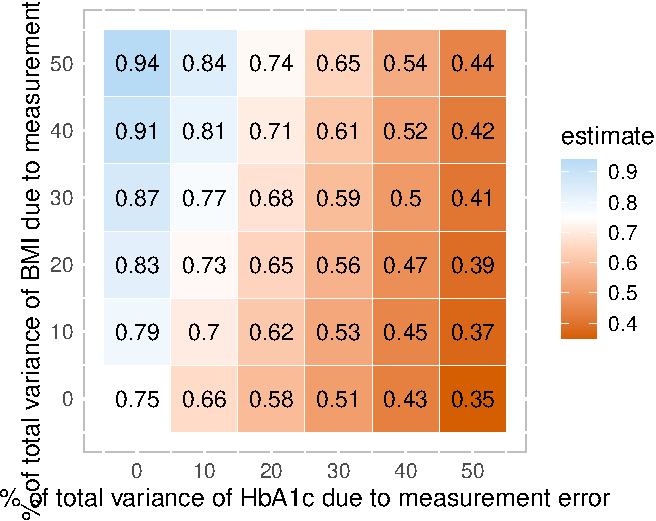
\includegraphics{manuscript_files/figure-pdf/unnamed-chunk-8-1.pdf}

}

\end{figure}

\begin{Shaded}
\begin{Highlighting}[]
\FunctionTok{ggsave}\NormalTok{(}\StringTok{"results/Figure\_STRATOS.tif"}\NormalTok{,}
       \AttributeTok{plot   =}\NormalTok{ FIGURE,}
       \AttributeTok{width  =} \DecValTok{6}\NormalTok{,}
       \AttributeTok{height =} \DecValTok{4}\NormalTok{,}
       \AttributeTok{dpi    =} \DecValTok{300}\NormalTok{,}
       \AttributeTok{units  =} \StringTok{"in"}\NormalTok{,}
       \AttributeTok{device =} \StringTok{"tiff"}\NormalTok{)}
\end{Highlighting}
\end{Shaded}

\hypertarget{refs}{}
\begin{CSLReferences}{1}{0}
\leavevmode\vadjust pre{\hypertarget{ref-boulesteix}{}}%
Boulesteix, Anne-Laure, Rolf H. H. Groenwold, Michal Abrahamowicz, et
al. 2020. {``Introduction to Statistical Simulations in Health
Research.''} \emph{BMJ Open} 10: e039921.
\url{https://doi.org/10.1136/bmjopen-2020-039921}.

\end{CSLReferences}



\end{document}
